Based on part (d), describe the solution $u(x, t)$ as time increases from a small value to a somewhat large value.
To illustrate your point, sketch the graphs of $u(x, t)$ for various $t$ and some fixed bar length $L_0$.

\begin{solution}\ \\\\
    As $t$ increases from a small value to a relatively large value, we observe that the temperature of the bar 
    uniformly reduces to that of the steady state solution, where the temperature at the insulated end 
    (which was initially the hottest) takes the longest to cool to that uniform steady state temperature. From (d), we
    know that the first (and to a much lesser degree, second) sine term dominates; since the period of this term is 
    twice that of the bar's length, we expect that the temperature curve should more or less be monotonically increasing
    with a uniform decrease effect as time goes on. In the figure below, we see precisely this; the plots for a single
    Fourier series term and for 10 terms differ only marginally where the temperature at $x = L$ is the highest for 
    each $t$.    

    \begin{figure*}[h]
        \centering
        \begin{subfigure}[b]{0.475\textwidth}
            \centering
            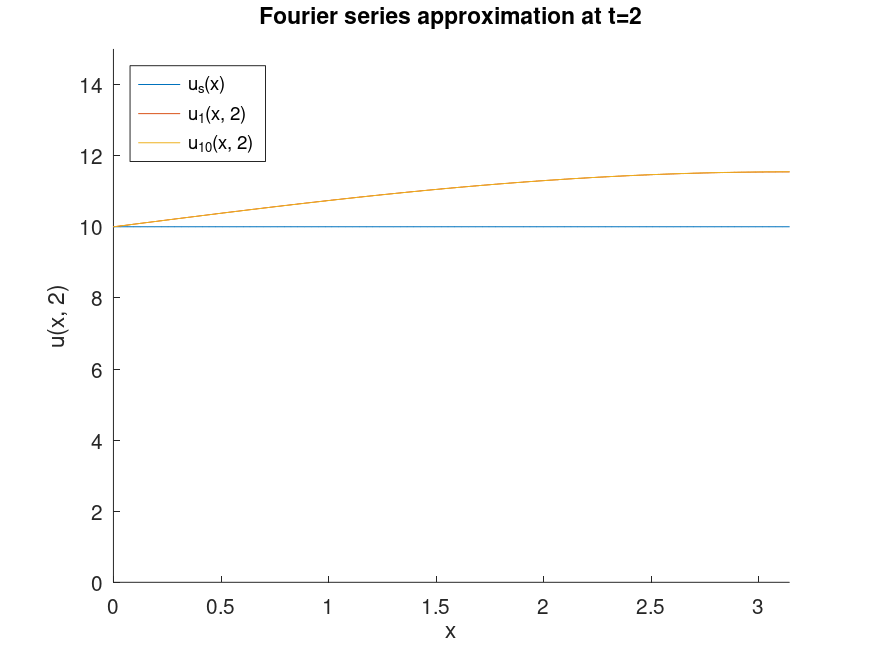
\includegraphics[width=\textwidth]{problem1e_fourier_series_solution_t_2.png}
            \label{fig:problem1e_t2}
        \end{subfigure}
        \hfill
        \begin{subfigure}[b]{0.475\textwidth}
            \centering
            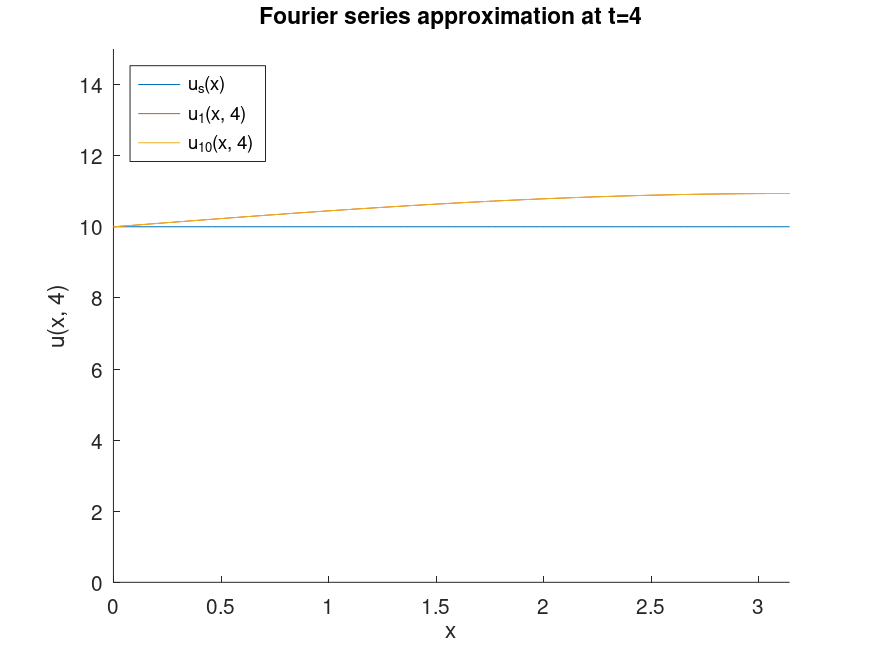
\includegraphics[width=\textwidth]{problem1e_fourier_series_solution_t_4.png}
            \label{fig:problem1e_t4}
        \end{subfigure}

        \centering
        \begin{subfigure}[b]{0.475\textwidth}
            \centering
            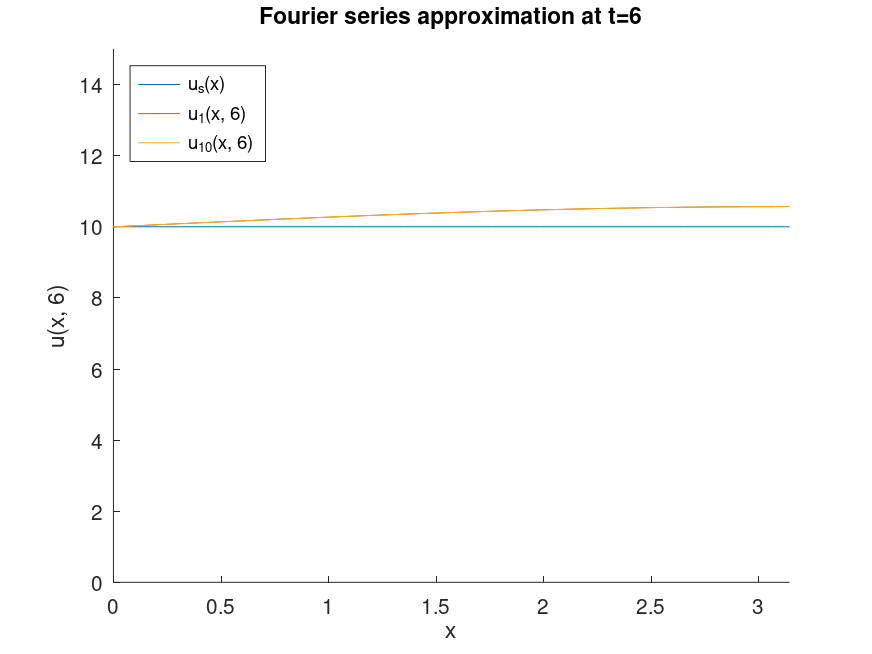
\includegraphics[width=\textwidth]{problem1e_fourier_series_solution_t_6.png}
            \label{fig:problem1e_t6}
        \end{subfigure}
        \hfill
        \begin{subfigure}[b]{0.475\textwidth}
            \centering
            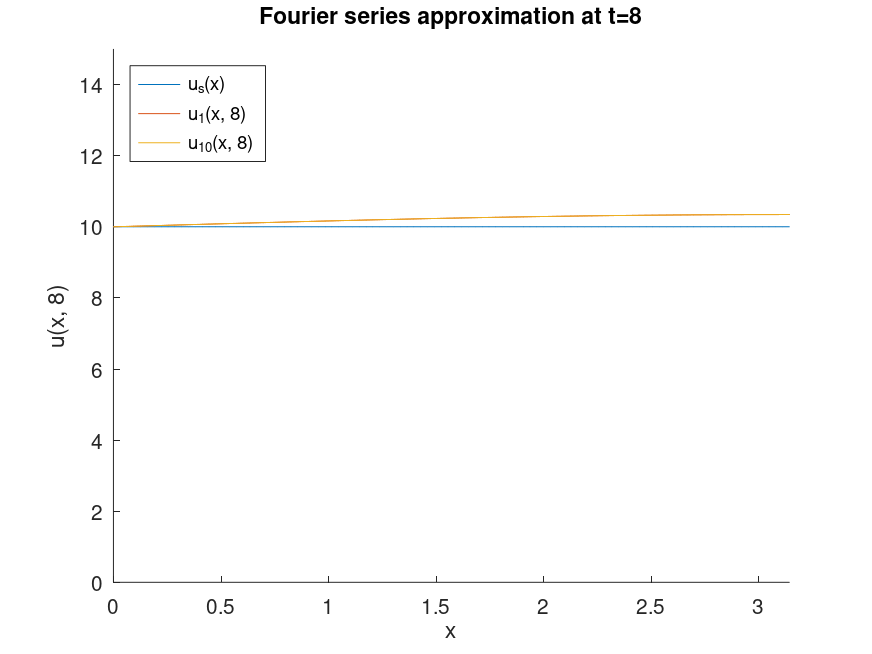
\includegraphics[width=\textwidth]{problem1e_fourier_series_solution_t_8.png}
            \label{fig:problem1e_t8}
        \end{subfigure}
        \caption[]{Fourier Series Approximations for various $t$}
    \end{figure*}
\end{solution}